\begin{frame}{Time representation}
\par \textbf{Objective}: Evolve multi-agent systems in order to naturally take into account the temporal dimension in the same way as the spatial and organisational dimensions
\vspace{.5cm}
\par \textbf{Proposition}:
\begin{itemize}
    \item A medium that allows the agents share and to access to information about the temporal activation dynamics
    \item \textbf{\st{A temporal knowledge representation model}
}
\end{itemize}
    
\note{
Notre première contribution concerne la représentation du temps dans les simulations multi-agent.
Notre objectif est de faire évoluer les simulations multi-agents de manière à prendre en compte naturellement la dimension temporelle au même titre que les dimensions spatiale et organisationnelle. Dans ce cadre, nous tenons à bien souligner que nous ne nous intéressons pas aux modèles de représentation de connaissances temporelles. Nous proposons un support permettant aux agents de partager et de percevoir des informations sur la dynamique temporelle.
}
\end{frame}

\begin{frame}{Time representation}{Proposition}
\begin{columns}
\begin{column}{.30\linewidth}
    \begin{figure}
	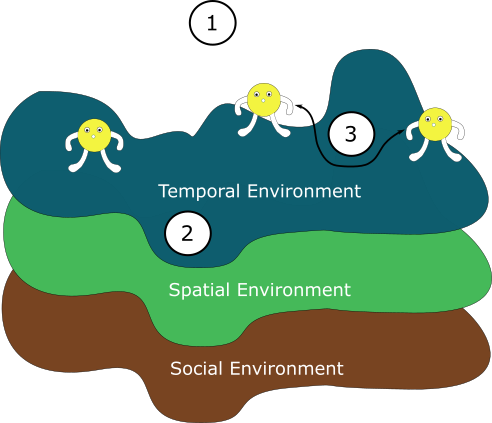
\includegraphics[width=1.2\textwidth]{figures/temporalRepresentation.png}
    \end{figure}
\end{column}
\begin{column}{.60\linewidth}
\begin{enumerate}
    \item The \textbf{Agent-Group-Role-Environment-Time (AGRET)} model : a MAS design methodology that articulates the spatial, organizational and temporal dimension
    \medbreak
    \item The \textbf{temporal environment} : an interaction environment for sharing, storing and perceiving temporal information
    \medbreak
    \item The \textbf{Influence-Reaction Model For Simulation (IRM4S)}: an interaction model that links the agents and the temporal environment
\end{enumerate}
\end{column}
\end{columns}
    
\note{
Pour mettre en place ce nouveau support au sein du système existant, nous proposons un ensemble de solutions axé sur trois points:
\begin{enumerate}
    \item une méthodologie de conception permettant d’articuler les 3 dimensions spatiale, organisationnelle et temporelle. Nous appelons cette approche AGRET.
    \item Un milieu d’interaction qui permet le stockage et l’accès aux informations temporelles. Nous appelons ce milieu environnement temporel.
    \item un modèle d’interaction qui permet le lien entre les agents et le milieu d’interaction. Nous utilisons un modèle existant : IRM4S, que nous appliquons à l'environnement temporel.
\end{enumerate}
Je vais donc présenter brièvement chaque solution.
}
    
\end{frame}

\begin{frame}{1. Agent-Group-Role-Environment-Time (AGRET)}
\par \textbf{Objective}: naturally and equally take the spatial, temporal and organizational dimensions into account

\par \textbf{Proposition}: The AGRET model consists of an extension and an enrichment of one of the most well-known and widely used organizational approaches in MAS: AGR and its extension AGRE.
\begin{itemize}
    \item AGR takes into account only the organizational dimension
    \item AGRE adds the \say{located in space} aspect to AGR: takes into account both the organisational and the spatial dimension equally
    \item AGRET adds the \say{located in time} aspect to AGRE: takes into account the organisational, spatial and temporal dimensions in the same way

\end{itemize}
    
\note{
Agent-Groupe-Rôle-Environnement-Temps est une approche qui prend en compte naturellement et au même titre les dimensions spatiale, temporelle et organisationnelle.
Elle se base sur une des approches organisationnelles les plus connus et la plus communément utilisée dans les SMA : AGR et de sa variante AGRE, que nous étendons et enrichissons. Il rajoute l'aspect situé dans le temps aux deux aspects situés dans l'espace et dans la dimension sociale d'\gls{agre}. \gls{agre} est elle-même une extension du modèle générique d'organisation \gls{agr}. Il ajoute la prise en compte de l'environnement spatial au modèle \gls{agr} qui ne considère que les organisations.
}
\end{frame}

\begin{frame}{1. Agent-Group-Role-Environment-Time (AGRET)}
\begin{figure}
	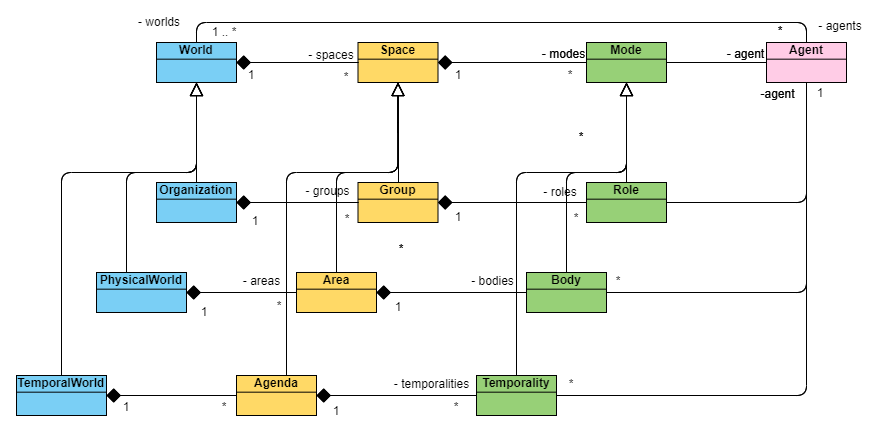
\includegraphics[width=\textwidth]{figures/agret.PNG}
\end{figure}
\note{
Voici le diagramme UML correspondant à notre modèle AGRET. Je vais vous montrer petit à petit l'évolution de ce modèle jusqu'à ce que nous proposons AGRET.
}
\end{frame}

\begin{frame}{1. Agent-Group-Role-Environment-Time (AGRET)}{AGR}
\begin{figure}
	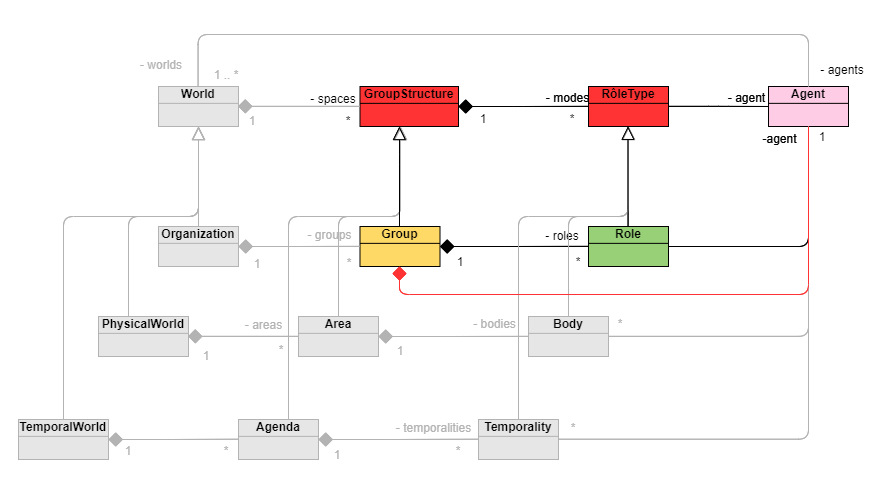
\includegraphics[width=\textwidth]{figures/agr.png}
\end{figure}

\note{
\par Le diagramme UML correspondant à AGR est celui qui n'est pas grisé. Le lien en rouge est propre à AGR. L’organisation d’AGR s'articule autour de trois notions : Agent, Groupe, Rôle
\begin{enumerate}
    \item Un agent est une entité active et communicante. 
    \item Un groupe est un ensemble d'agents partageant des caractéristiques communes. 
    \item Un rôle est la représentation abstraite d'une position fonctionnelle d'un agent dans un groupe.
\end{enumerate}
Un agent joue un rôle dans un ou plusieurs groupes, peut tenir plusieurs rôles et peut être membre de plusieurs groupes.
}
\end{frame}

\begin{frame}{1. Agent-Group-Role-Environment-Time (AGRET)}{AGRE}
\begin{figure}
	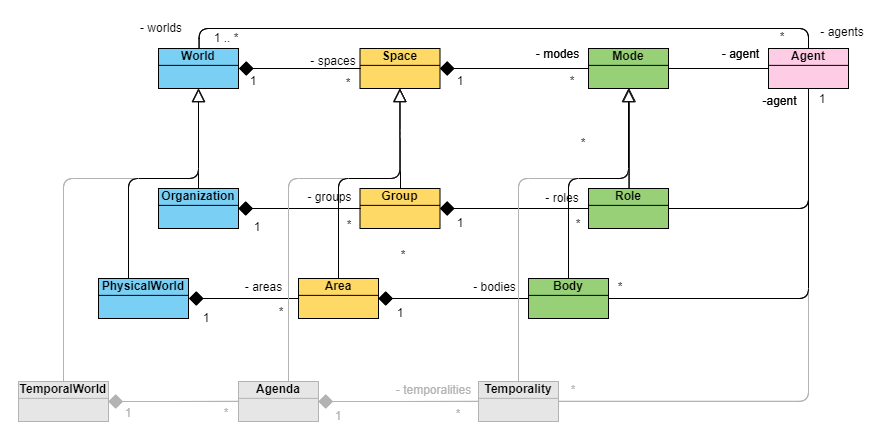
\includegraphics[width=\textwidth]{figures/agre.png}
\end{figure}

\note{
AGRE vient alors compléter l’aspect situé corporel à l’aspect situé social d'AGR. AGRE défini, en plus du concept d'agent, trois concepts généraux qui se déclinent en concepts spécifiques selon le type d'environnement (organisationnel ou spatial) :
\begin{enumerate}
    \item Un espace est un domaine dans lesquels les agents sont situés.
    \item Un mode est la manifestation d'un agent dans un domaine spécifique, son mode d'existence et son apparence dans un espace. Un mode décrit la position de l'agent et la manière dont il perçoit et agit dans un space.
    \item Un monde est une collection de spaces de même type. 
\end{enumerate}
AGRE définit deux types de mondes : les organisations qui représentent l'environnement social et qui sont composées de groupes et le monde physique qui représente l'environnement physique et qui est composé de zones. Les agents sont alors situés dans les spaces et peuvent y agir à travers les modes. Un mode dans une zone est appelé corps (body) tandis qu'un mode dans un groupe est appelé rôle (role).
Dans leur article  Ferber et al. considèrent uniquement deux types de monde. Néanmoins, ils évoquent la possibilité d'existence d'autres types de monde et d'autres types d'espace qu'ils ne décrivent pas dans leur article. 

}
\end{frame}

\begin{frame}{1. Agent-Group-Role-Environment-Time (AGRET)}
\begin{figure}
	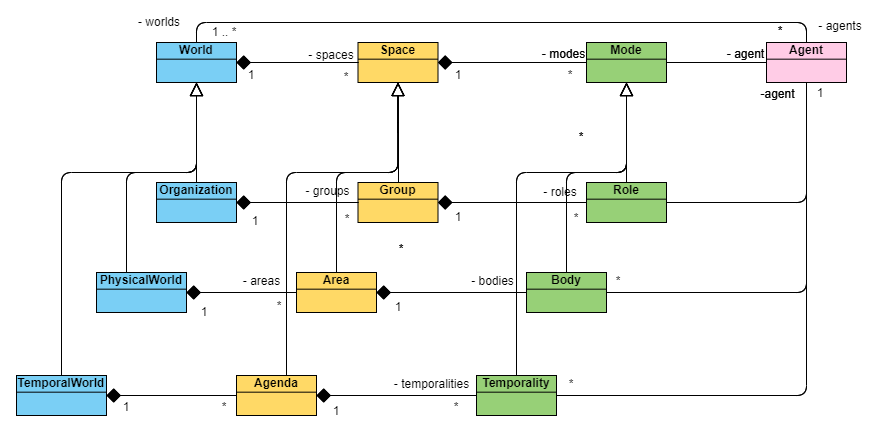
\includegraphics[width=\textwidth]{figures/agret.PNG}
\end{figure}
\medbreak
\par \textbf{Originality}: Consideration of the temporal dimension as a medium of interaction, \alert{the temporal environment}
    
\note{
Dans AGRET, nous reprenons les principes de base d'AGRE et nous ajoutons la dimension temps. Nous définissons alors un nouveau type d'espace qui est de type temporel et que nous appelons agenda. Comme dans AGR et AGRE, les agents sont situés dans les espaces et peuvent y agir à travers les modes. Si un mode dans une zone est appelé corps (body), un mode dans un groupe est appelé rôle (role), nous appelons un mode dans un agenda une  temporalité (temporality). Un nouveau type de monde vient également s'ajouter à ces deux types de monde déjà existants dans AGRE: le monde temporel (temporal world).
La figure montre un diagramme UML simplifié qui représente les relations entre mondes, espaces, zones, groupes, agendas, modes, corps, rôles et temporalités.

\par Une des originalités de notre proposition, comparée à d'autres approches de gestion du temps est la représentation du temps simulé comme un milieu d'interaction. Nous avons appelé ce milieu d'interaction environnement temporel. Cet environnement temporel vient en complément à l'ordonnanceur de la simulation. 
}
\end{frame}

\begin{frame}{2. The Temporal Environment}{An interaction medium}
\par \textbf{Observation}: Most of the time, the spatial and organizational dimensions are modeled as environments
\medbreak
\par \textbf{Proposition} : modelling the temporal dimension as an environment called the \textbf{temporal environment} 
\medbreak
\begin{block}{Remarks}
The temporal environment does not replace the scheduler but complements its role
\begin{itemize}
    \item It comes between the scheduler and the agent
    \item It breaks the direct link between the agent and the scheduler
\end{itemize}
\vspace{.3cm}
\par The the temporal dimension management is done on two levels
\begin{itemize}
    \item \textbf{Temporal environment}: representation of temporal dynamics, exchange
    \item \textbf{Scheduler}: management of the simulation activation cycle
\end{itemize}
\end{block}
    
\note{
En partant du constat que les dimensions spatiale et organisationnelle sont modélisé, la plupart du temps, sous forme d’environnements, nous proposons une modélisation du temps sous forme d’environnement. Nous appelons cet environnement : l’environnement temporel. Il s’agit d’un espace dont la métrique est le temps.
Nous tenons tout de même à noter que l’environnement temporel ne remplace pas l’ordonnanceur de la simulation, il  vient compléter son rôle. L’environnement temporel vient s’interfacer entre l’agent et l’ordonnanceur cassant le lien direct entre ces derniers.
La gestion de la dimension temporelle se fait alors sur deux niveaux:
\par L’environnement temporel gère la représentation de la dynamique d’activation temporelle des agents ainsi que les échanges d’informations sur cette dimension temporelle
\par L’ordonnanceur gère le cycle d’activation de la simulation
Nous reviendrons plus en détails sur ces deux niveaux lorsque nous aborderons l’aspect modèle d’interaction.
}
\end{frame}

\begin{frame}{2. The Temporal Environment}{An Interaction Medium}
\par \textbf{Structure and mechanics} based on the Temporality Model
\vspace{.5cm}
\begin{block}{Temporality Model}
\begin{itemize}
    \item  A time scheduling approach (used only by the scheduler)
    \item Research work of our CAS working group (Dr. Payet)
\end{itemize}
\end{block}
\vspace{.5 cm}
\par \textbf{Proposition}: redesign the temporality model in order to reuse its basic principles in the structuring and the implementation of the temporal environment mechanics
\medbreak
\Centering{
\par Use of the temporality model in the level of:\\
the scheduler (Dr Payet) \alert{$\ne$} the temporal environment (My thesis)}


\note{
Un environnement possède une structure, un ensemble de mécaniques et une dynamique qui lui sont propre. La structure et les mécaniques propres à l’environnement temporel se basent sur les principes du modèle à temporalité. Le modèle à temporalité est une approche qui à l’origine était utilisé uniquement au niveau de l’ordonnancement de la simulation, au même titre que l’approche à pas de temps constant, l’approche événementielle ou l’approche hybride. Elle fait partie des contributions de notre équipe de recherche, plus précisément des travaux de Mr Payet. Dans cette thèse, je procède à une refonte du modèle pour une réutilisation de ses principes de base dans la structuration et la mise en place des mécaniques de l’environnement temporel. Il est donc très important de bien distinguer l’utilisation de l’approche de type modèle à temporalité pour l’ordonnancement de la simulation et de sa réutilisation pour la structuration et la mise en place des mécaniques de l’environnement temporel. Cette deuxième fait partie des contributions de cette thèse.
}
    
\end{frame}

\begin{frame}{2. The Temporal Environment}{An Interaction Medium}
\textbf{Use of the temporality model at the level of the \alert{scheduler}}
\begin{itemize}
    \item A particular type of time scheduling approach
    \item An expressive approach: allows the agent to describe his own temporal dynamics (sharing of temporal information)
    \item Integrates a support that allow representing this dynamic in the form of:
\end{itemize}

\begin{figure}
	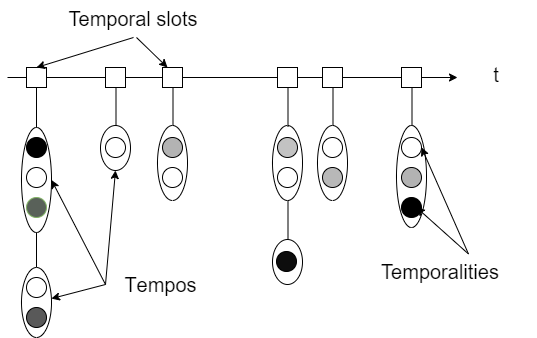
\includegraphics[width=.5\textwidth]{figures/temporalityModel.png}
\end{figure} 
\par \textbf{Limit}: allows neither the storage of temporal information nor its access
\note{
\footnotesize{Comparée aux autres approches d'ordonnancement du temps, nous pensons que le modèle à temporalité est intéressante pour la structuration de l'environnement temporelle car
\par C'est une approche expressive: ie, elle permet aux agents de définir eux-mêmes et de partager leur dynamique d'activation temporelle.
\par De plus , elle intègre également un support permettant de représenter cette dynamique sous forme de temporalités, tempos, d'axe temporel et de slots temporels. Dans le modèle à temporalité, l'agent indique à l’ordonnanceur de la simulation à quelle moment il souhaite être réveillé ou activé en définissant une structure de donnée appelée temporalité. Le traitement interne des temporalités par l'ordonnanceur fait intervenir deux structures de données: le slot temporel et le tempo. L’ordonnanceur fait progresser  le temps simulé  en l’emmenant successivement sur chacune des positions signalées par un slot temporel.
\par Nous avons donc là une approche qui permet le partage et la structuration des informations temporelles. Cependant, cette mécanique ne permet ni le stockage des informations ni leur perception.
\par En effet, les temporalités passées sont supprimés car elles n'interviennent plus dans le cycle d'activation de la simulation et l'ordonnanceur calcule les prochaines dates de déclenchement des temporalités futures avant chaque avancement du temps. Il s'agit d'un comportement tout à fait normal compte tenu de l'objectif qui est l'ordonnancement du temps.
\par Cependant, le stockage et la perception des informations sont indispensables au niveau de l'environnement temporel. Nous procédons alors à une refonte du modèle en intégrant notamment ces possibilités.

}
}
\end{frame}

\begin{frame}{2. The Temporal Environment}{An Interaction Medium}
\textbf{Use of the (modified version of) temporality model at the level of the \alert{temporal Environment}}
\begin{itemize}
    \item Structure : time axis, tempo, temporal slot, etc.
    \item Environmental Mechanics
\end{itemize}
%\vspace{.5cm}
\begin{table}[]
\resizebox{\textwidth}{!}{%
\begin{tabular}{ll}
\hline
\rowcolor[HTML]{34495E} 
{\color[HTML]{FFFFFF} Scheduler}                     & {\color[HTML]{FFFFFF} Temporal Environment}                                                                                                                                                                                     \\ \hline
\multicolumn{1}{|c|}{-}                              & \multicolumn{1}{l|}{\alert{Temporality}: representation of the agent in the temporal environment}                                                                                                                                      \\ \hline
\multicolumn{1}{|l|}{\alert{Temporality} $t=\{id,d,f,p,v\}$} & \multicolumn{1}{l|}{\begin{tabular}[c]{@{}l@{}}\\[.2cm]\alert{Temporal location} $l=\{\underbrace{id,d,f,p,v}_{Mandatory\ parameters} ,\underbrace{...}_{optional\  parameters}\}$\\[1cm] * Optional parameters. Ex: queue, cost, criticality, priority, accessibility, etc.\end{tabular}} \\ \hline
\multicolumn{1}{|l|}{Temporal Slot}                  & \multicolumn{1}{l|}{Temporal Slot}                                                                                                                                                                                              \\ \hline
\multicolumn{1}{|l|}{Tempo}                          & \multicolumn{1}{l|}{Tempo}                                                                                                                                                                                                      \\ \hline
\multicolumn{1}{|l|}{\begin{tabular}[c]{@{}l@{}}No storage:\\ - The next activation dates of future temporalities \\ are calculated before each advance of time\\ - Temporalities are removed after activation\end{tabular}}                          &
\multicolumn{1}{l|}{\begin{tabular}[c]{@{}l@{}}- Storage of past, present and future information\\ - Storage Time Window $\Delta_s=[\delta_{smin}, \delta_{smax}]$\end{tabular}} \\ \hline
\multicolumn{1}{|l|}{
No possibility of collecting information}                                                                                                                                                                              & 
\multicolumn{1}{l|}{Ability to perceive past, present and future information}                                                                                                   \\ \hline
\end{tabular}
}
\caption{Use of the temporality model at the scheduler level and at the level of the temporal environment: comparison and equivalence }
\end{table}


    
\note{\footnotesize{Ce tableau présente les correspondances entre les principes de bases de l’approche de type modèle à temporalité lorsqu’ils sont utilisé pour l’ordonnancement de la simulation et lorsque nous ré-adaptons pour une utilisation dans le cadre de l’environnement temporel.
\par Dans l’environnement temporel, une temporalité est la représentation de l'agent dans l'environnement temporel,  au même titre que le corps de l'agent dans l'environnement spatial ou le rôle dans l'environnement social. Cette notion est propre à l'environnement temporel. Il n'a donc pas d'équivalent au niveau de l'ordonnanceur. Le corps possède une localisation spatiale dans l'environnement physique. Son déplacement se traduit par la modification de sa localisation spatiale. De la même manière, une temporalité possède une localisation temporelle dans l'environnement temporel. Son déplacement se traduit par la modification de sa localisation temporelle. C'est cette notion de localisation temporelle dans l'environnement temporel qui est équivalente à la notion de temporalité dans le modèle à temporalité au niveau de l'ordonnanceur. 
\par Cette localisation temporelle est définie par un ensemble de paramètres obligatoires et des paramètres optionnels qui peuvent être ajoutés en fonction des besoins du modèle. Par exemple, dans notre cadre applicatif, nous ajoutons l'estimation de la longueur de la file d'attente, le cout correspondant, etc. comme paramètre optionnel.
\par Les notions de tempo et de slot temporels quant à eux restent les mêmes.
\par Nous mettons également en place un le stockage et la perception des information positionnées sur le passé, sur le présent et sur le futur. 
\par Par ailleurs, la pertinence de ces informations varie en fonction du temps, du modèle et du type d'information. Une information passée peut avoir une durée de vie au-delà de laquelle elle devient obsolète. De même, au-delà d'une certaine limite dans le temps, une information future n'est pas forcément pertinente. Nous mettons en place un horizon temporel de stockage  dont les valeurs des bornes sont définies arbitrairement par l'utilisateur ou le concepteur du modèle.
\par
}
}
\end{frame}

\begin{frame}{2. The Temporal Environment}{An Interaction Medium}
\alert{Remarks:}
\begin{itemize}
    \item The readaptation of the basic principles of the temporal model for use in the temporal environment is \textbf{completely independent} of the scheduling approach used in the scheduler of the simulation
    \item We can set up a temporal environment that can be coupled with a scheduler that uses another type of approach: time-stepped, event-driven, etc.

\end{itemize}
\note{
Il est important de noter que la ré-adaptation des principes de bases du modèle à temporalité pour une utilisation au niveau de l’environnement temporel est tout à fait indépendante de l’approche d’ordonnancement utilisé au niveau de l’ordonnanceur de la simulation. Ainsi, il est tout à fait possible de mettre en place un environnement temporel que l’on couple avec un ordonnanceur qui utilise un autre type d’approche : à pas de temps constant, événementielle, etc.

}
\end{frame}

\begin{frame}{3. IRM4S}{An Interaction Model}
2 types of interaction models:
\begin{itemize}
    \item Action/Reaction: \footnote{$Behaviour_a$ describes the activation cycle of the agent $a$ : perception, deliberation, action or influence }$Behaviour_a :\footnote{$\Sigma$ is the environment state}\Sigma \mapsto \Sigma$
    \item Influence/Reaction: $Behaviour_a: \footnote{$\Gamma$ is an influence : does not directly change the state of the environment. It represents an agent's desire to see it changed in some way}\Gamma \mapsto \Gamma$
\begin{itemize}
    \item Compliance with the environmental integrity constraint
    \item Respect for the autonomy of the agents
    \item Reduction of the agent-action-environment coupling: the simulation is less sensitive to the way it is implemented
    \item Clearly distinguishes between agent and environment
\end{itemize}
\end{itemize}
\textbf{IRM4S}: $ Behaviour_a: \Sigma \times \Gamma \mapsto \Gamma$
\begin{itemize}
    \item Approach adapted to multi-agent simulation
    \item Takes into account an agent's local and subjective perception of his environment
\end{itemize}
\note{

Maintenant, je vais vous introduire le modèle d’interaction qui permet de définir le lien entre l’agent et l’environnement. Ce lien se traduit par le fait que l’agent perçoit son environnement et agit sur ce dernier. 
\par Nous choisissons d'utiliser IRM4S qui 
simplification” et une clarification du modèle influence/réactio dans le cadre de la simulation multi-agent. Comme dans toute approche de type i/r, le cycle comportemental de l'agent, traduit par la fonction behaviour, aboutit à la production d'influences. Cependant, dans le modèle i/r, les agents perçoivent ce qui les influence, mais ne sont pas influencés par l'état de l'environnement.
\par Contrairement à cela, IRM4S prend en compte la perception locale et subjective de son environnement par un agent. Nous utilisons IRM4S dans le cadre de la mise en place de l’environnement temporel.

%Il existe deux types de modèles d’interactions communément utilisé dans les SMA. Nous choisissons de nous pencher sur un modèle i/r car il respecte la contrainte d’intégrité environnementale et la propriété d’autonomie des agents du système. Il permet donc de réduire le couplage entre agent-action-environnement. Ainsi, le modèle est moins sensible à la manière dont il est implémenté. 
%\par Le cycle comportemental classique d’un agent se résume en trois phases: perception, délibération, action ou influence. Ce cycle est traduit par une fonction $Behaviour_a$. Dans l'approche a/r, il aboutit à une transformation directe de l’environnement. Contrairement à cela, dans le modèle i/r, il aboutit à une influence. L'influence diffère de l’action dans le sens où elle ne modifie pas directement l'environnement. Elle représente le souhait d'un agent de le voir modifié d'une certaine façon. Ce modèle distingue alors bien tout ce qui relève de l’agent de tout ce qui relève de l’environnement. En d'autres termes, un agent ne peut que décider de l'action suivante à faire. C'est à son environnement de déterminer les conséquences de cette dernière. Par exemple : un agent décide de faire déplacer un objet de l’environnement, mais c'est son environnement (son corps et son environnement extérieur) qui exécute le déplacement.
%\par Ferber et al. proposent une “simplification” et une clarification du modèle i/r dans le cadre de la simulation multi-agent. Le modèle s'appelle IRM4S. Il s'agit d'une approche adaptée dans un contexte de simulation multi-agent.
%\par Comme dans toute approche de type i/r, dans IRM4S le cycle comportemental de l'agent aboutit à la production d'influences. Cependant, dans le modèle i/r, les agents perçoivent ce qui les influence, mais ne sont pas influencés par l'état de l'environnement. \par Contrairement à cela, IRM4S prend en compte la perception locale et subjective de son environnement par un agent. Nous utilisons IRM4S dans le cadre de la mise en place de l’environnement temporel.
}

\end{frame}

\begin{frame}{3. IRM4S}{An Interaction Model}
\pa The introduction of the temporal environment induces consequences on 2 levels:
\begin{enumerate}
    \item The agent activation cycle
    \item The simulation activation cycle
\end{enumerate}

\begin{block}{The agent activation cycle}
\par Perception time window $\Delta_{pt}=[\delta_{ptmin},\delta_{ptmax}]$ (the agent has a limited perception of its environment)
\vspace{.5cm}
\begin{equation*}
    Perception:\Sigma \times \Gamma \times  \footnote{Temporal, spatial, social perception window}\alert{\Delta_p} \mapsto P
\end{equation*}

\end{block}

\note{

\par L'introduction de l'environnement temporel induit des conséquences au niveau du modèle d'intéraction sur 2 niveaux:
\begin{enumerate}
    \item Au niveau du cycle d'activation des agents
    \item Au niveau du cycle d'activation de la simulation
\end{enumerate}
\par Au niveau du cycle d'activation des agents: pour chaque agent ou chaque type d'agent, nous définissons une fenêtre temporelle ou horizon temporel de perception noté $\Delta_p=[\delta_{pmin},\delta_{pmax}]$ . Cette horizon temporelle contraint la perception et traduit une propriété de l'agent : celle d'avoir une perception limitée de son environnement temporel. Il s'agit de l'équivalent temporel du champ de vision dans l'environnement spatial. 
La perception est donc donnée par la fonction suivante
où $\Sigma$ est l'état de l'environnement, $\Gamma$ est un ensemble d'influences, $\Delta_p$ est la fenêtre temporelle de perception et $P$ est un ensemble de percepts. 
\par Nous pouvons notamment noter la prise en compte, de manière explicite, de les horizons de perception dans la formalisation de la perception.
}
\end{frame}

\begin{frame}{3. IRM4S}{An Interaction Model}
\begin{block}{The simulation activation cycle}

\par \alert{Classical} simulation activation cycle:
\begin{enumerate}
    \item \textbf{environments activation}: These environments have states that evolve over time according to their own inertial laws, and the influences exerted by the agents : \textbf{time constrained environment}
    \item \textbf{agents activation}
\end{enumerate}
\vspace{.5cm}
\par \alert{New} simulation activation cycle:
\begin{enumerate}
    \item \textbf{time-constrained environments activation} phase over the time interval $]t-dt; t]$. Example : spatial environment, social environment
    \item \textbf{agents activation} phase on the current time time $t$;
    \item \textbf{non-constrained environments} activation phase on the consideration that $t$ is over. Example : temporal environment
    \begin{itemize}
        \item The temporal environment state determines the temporal dynamics
        \item The state of the temporal environment evolves out of time
    \end{itemize}
\end{enumerate}

\end{block}

\note{
\par Au niveau du cycle d'activation de la simulation: Dans la plupart des simulateurs, la phase d'activation de l'environnement se déroule en début du cycle d'activité de la simulation. Cela est dû au fait que la plupart des environnements a besoin de calculer son nouvel état en début d'un cycle (instant $t$), avant l'activation des agents. Ces calculs doivent  s'établir sur l'intervalle de temps qui s'est écoulé depuis la dernière activation. Ces environnements ont des états qui évoluent dans le temps en fonction des lois inertielles qui leur sont propres, et des influences qu'exercent les agents. Ce sont donc, en quelque sorte, des environnements contraints par le temps.
\par Dans notre contexte, la mise en place d'un nouveau type d'environnement qui est l'environnement temporel vient chambouler le fonctionnement de ce cycle classique d'ordonnancement de la simulation. Par définition, l'état de l'environnement temporel détermine la dynamique d'écoulement du temps. Par conséquent, son état évolue hors du temps. \textbf{L'environnement temporel n'est pas un environnement contraint par le temps}. 
Ainsi, aux deux phases du cycle d'activation classique de la simulation s'ajoute alors une troisième phase : la phase d'activation des environnements non contraints par le temps sur la considération que $t$ vient d'être passé.


}
\end{frame}

\begin{frame}{Summary}
\begin{figure}
	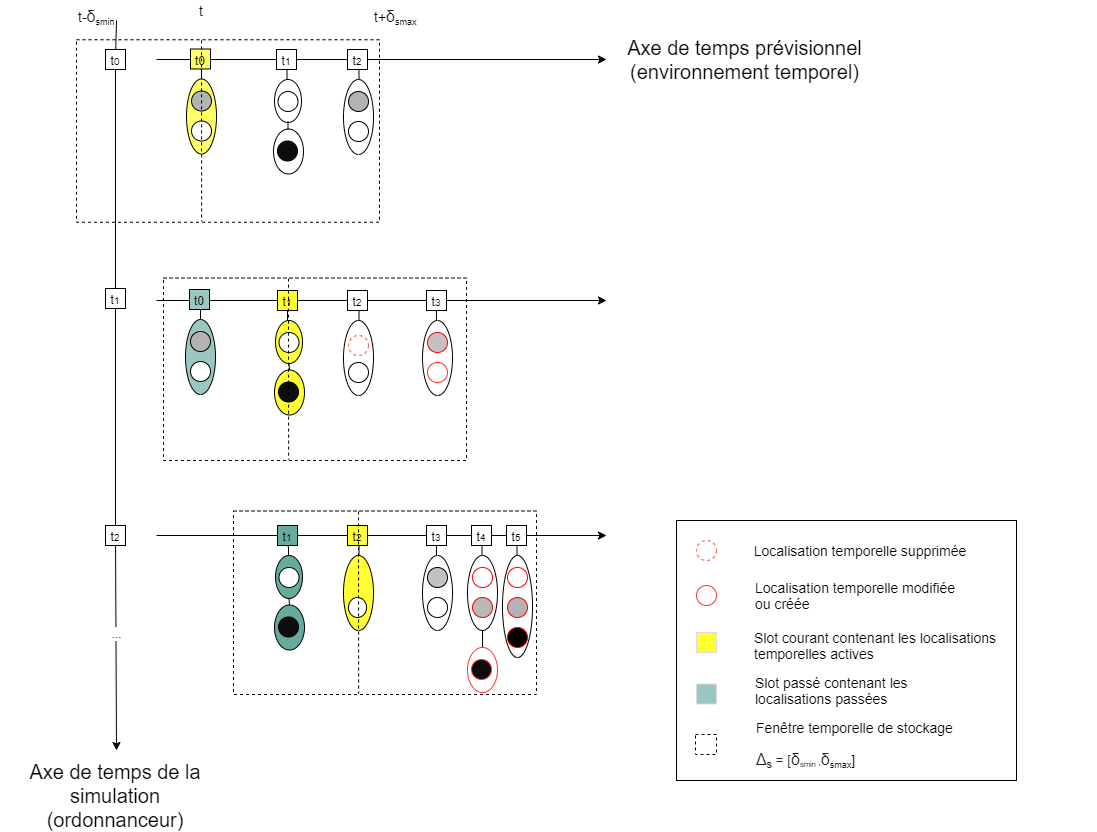
\includegraphics[width=.7\textwidth]{figures/EnvironnementTemporel.png}
	\caption{State of the temporal environment at each advance in time}
	\end{figure}

\note{Pour résumer, le schéma suivant illustre l’état (statique) de l’environnement temporel à chaque avancement du temps simulé: Cet état est donné par l’ensemble des localisations temporelles définies par tous les agents du système.
Nous distinguons notamment deux axes : 
l’axe de temps de la simulation qui correspond à l’horloge globale de la simulation et qui est gérée par l’ordonnanceur,
 l’axe de temps prévisionnel qui est l’axe de temps stocké au niveau de l’environnement temporel et qui traduit la dynamique prévisionnelle d’activation des agents. Cet axe de temps prévisionnel contient des localisations temporelles passées, présentes et futures.
}
\end{frame}

\begin{frame}{Summary}
	\begin{figure}
	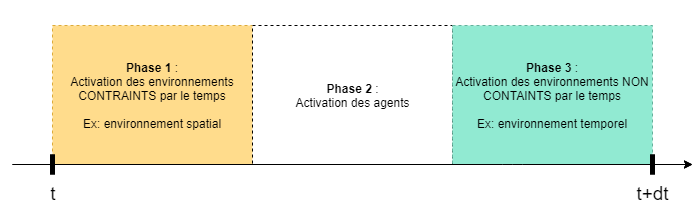
\includegraphics[width=\textwidth]{figures/Cycle_activite.png}
	\caption{New simulation activation cycle}
	\end{figure}
	
\note{
 \par L'introduction de l'environnement temporel conduit à l'ajout d'une 3ème phase au cycle d'activation de la simulation : la phase d'activation des environnements non-contraints par le temps.

}
\end{frame}

\begin{frame}{Implementation}
    \begin{figure}
	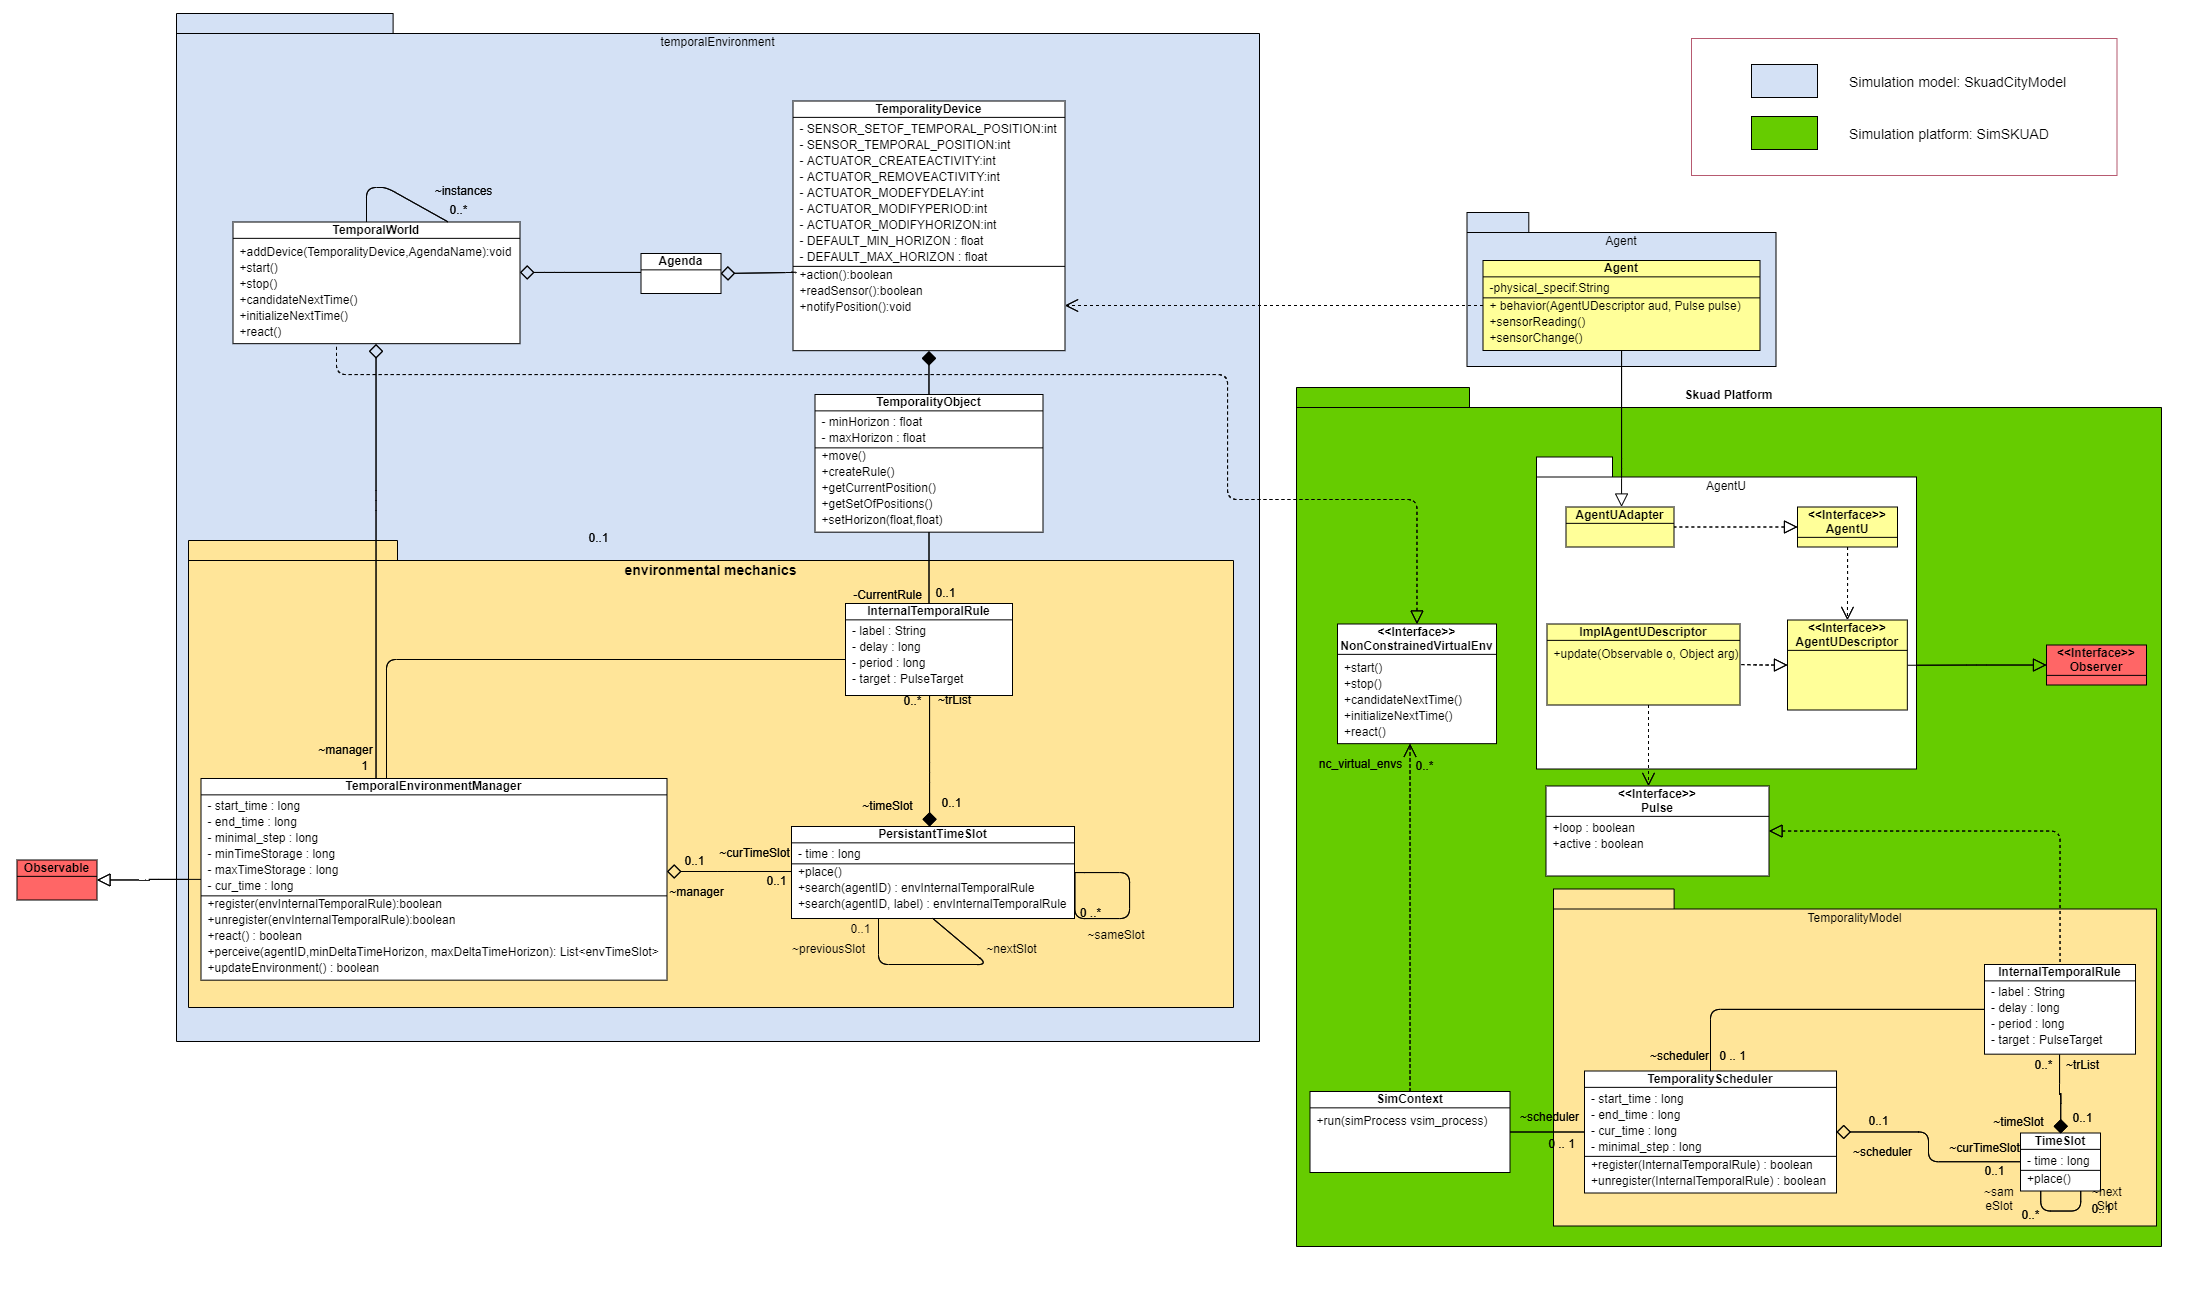
\includegraphics[width=\textwidth]{figures/temporalEnvironmentImpl.png}
	\end{figure}
\note{
Dans SkuadCitymodel, l’implémentation de notre première contribution s’effectue sur deux niveaux:
\begin{itemize}
    \item au niveau du modèle de simulation : implémentation de l’environnement temporel. 
    \item au niveau de la plateforme de simulation : mise à jour du mécanisme de gestion du cycle d’activation de la simulation. La mise en oeuvre au niveau de la plateforme de simulation, plus précisément au niveau de l’ordonnanceur consiste en la modification du cycle d’activation de la simulation afin de respecter les 3 phases que j’ai présenté précédemment: nous avons notamment mis en place la mise à jour des environnements non-contraints par le temps en début de cycle.
\end{itemize}
L’implémentation de l’environnement temporel au niveau du modèle de simulation se divise en deux parties:
\begin{itemize}
    \item la mise en oeuvre de la structure de l’environnement sur la base du modèle AGRET
    \item les mécaniques environnementaux
\end{itemize} 

}
\end{frame}

\begin{frame}{Implementation}{Structure}
2 types of environment in SimSKUAD:
\begin{enumerate}
    \item Physical
    \begin{itemize}
        \item the link between the agent and its representation in the environment is made by cabling using a physical slot
        \item Agent representation: body + device (integrates sensors and actuators)
        \item Ex : spatial environment, \textbf{temporal environment}
    \end{itemize}
    \item Social
    \begin{itemize}
        \item the link between the agent and the environment is made by cabling using a social slot
        \item Agent representation: avatar
        \item Ex : social environment
    \end{itemize}
\end{enumerate}
\vspace{.5cm}
\centering{\alert{The temporal environment} is implemented in the form of a \alert{physical environment.}}

\note{Dans tout modèle de simulation développé sur SimSKUAD, nous distinguons deux types d’environnements : l’environnement physique et l’environnement social. Techniquement parlant, l’environnement est dit physique lorsque le lien entre l’agent et sa représentation dans l’environnement se fait par cablâge via un slot physique. Cela lui permet de disposer d’une représentation physique et d’une entité que nous appelons device. Le device est un objet de l’environnement, des dispositifs matériels intégrant des capteurs et des actionneurs que les agents utilisent pour interagir avec un environnement physique. L’environnement est dit social lorsque le lien entre l’agent et l’environnement se fait par cablâge via un slot social. Cela lui permet de disposer d’une représentation dans l’environnement social appelée avatar. Pour faire simple, un avatar est un objet qui fournit des outils permettant d'opérer des modifications sur la dimension sociale (communiquer par message par exemple). L’environnement temporel est mise en oeuvre sous la forme d’un environnement physique. Cela permet à l’agent de disposer d’une temporalité qui est composé d'un corps et d’une device temporel qui intègre les capteurs et les actionneurs nécessaires à la manipulation de l’environnement temporel par les agents. Nous avons également sur le schéma l’espace qui est l’agenda et le monde temporel.}
    
\end{frame}

\begin{frame}{Implementation}{Environmental mechanics}
    \begin{figure}
	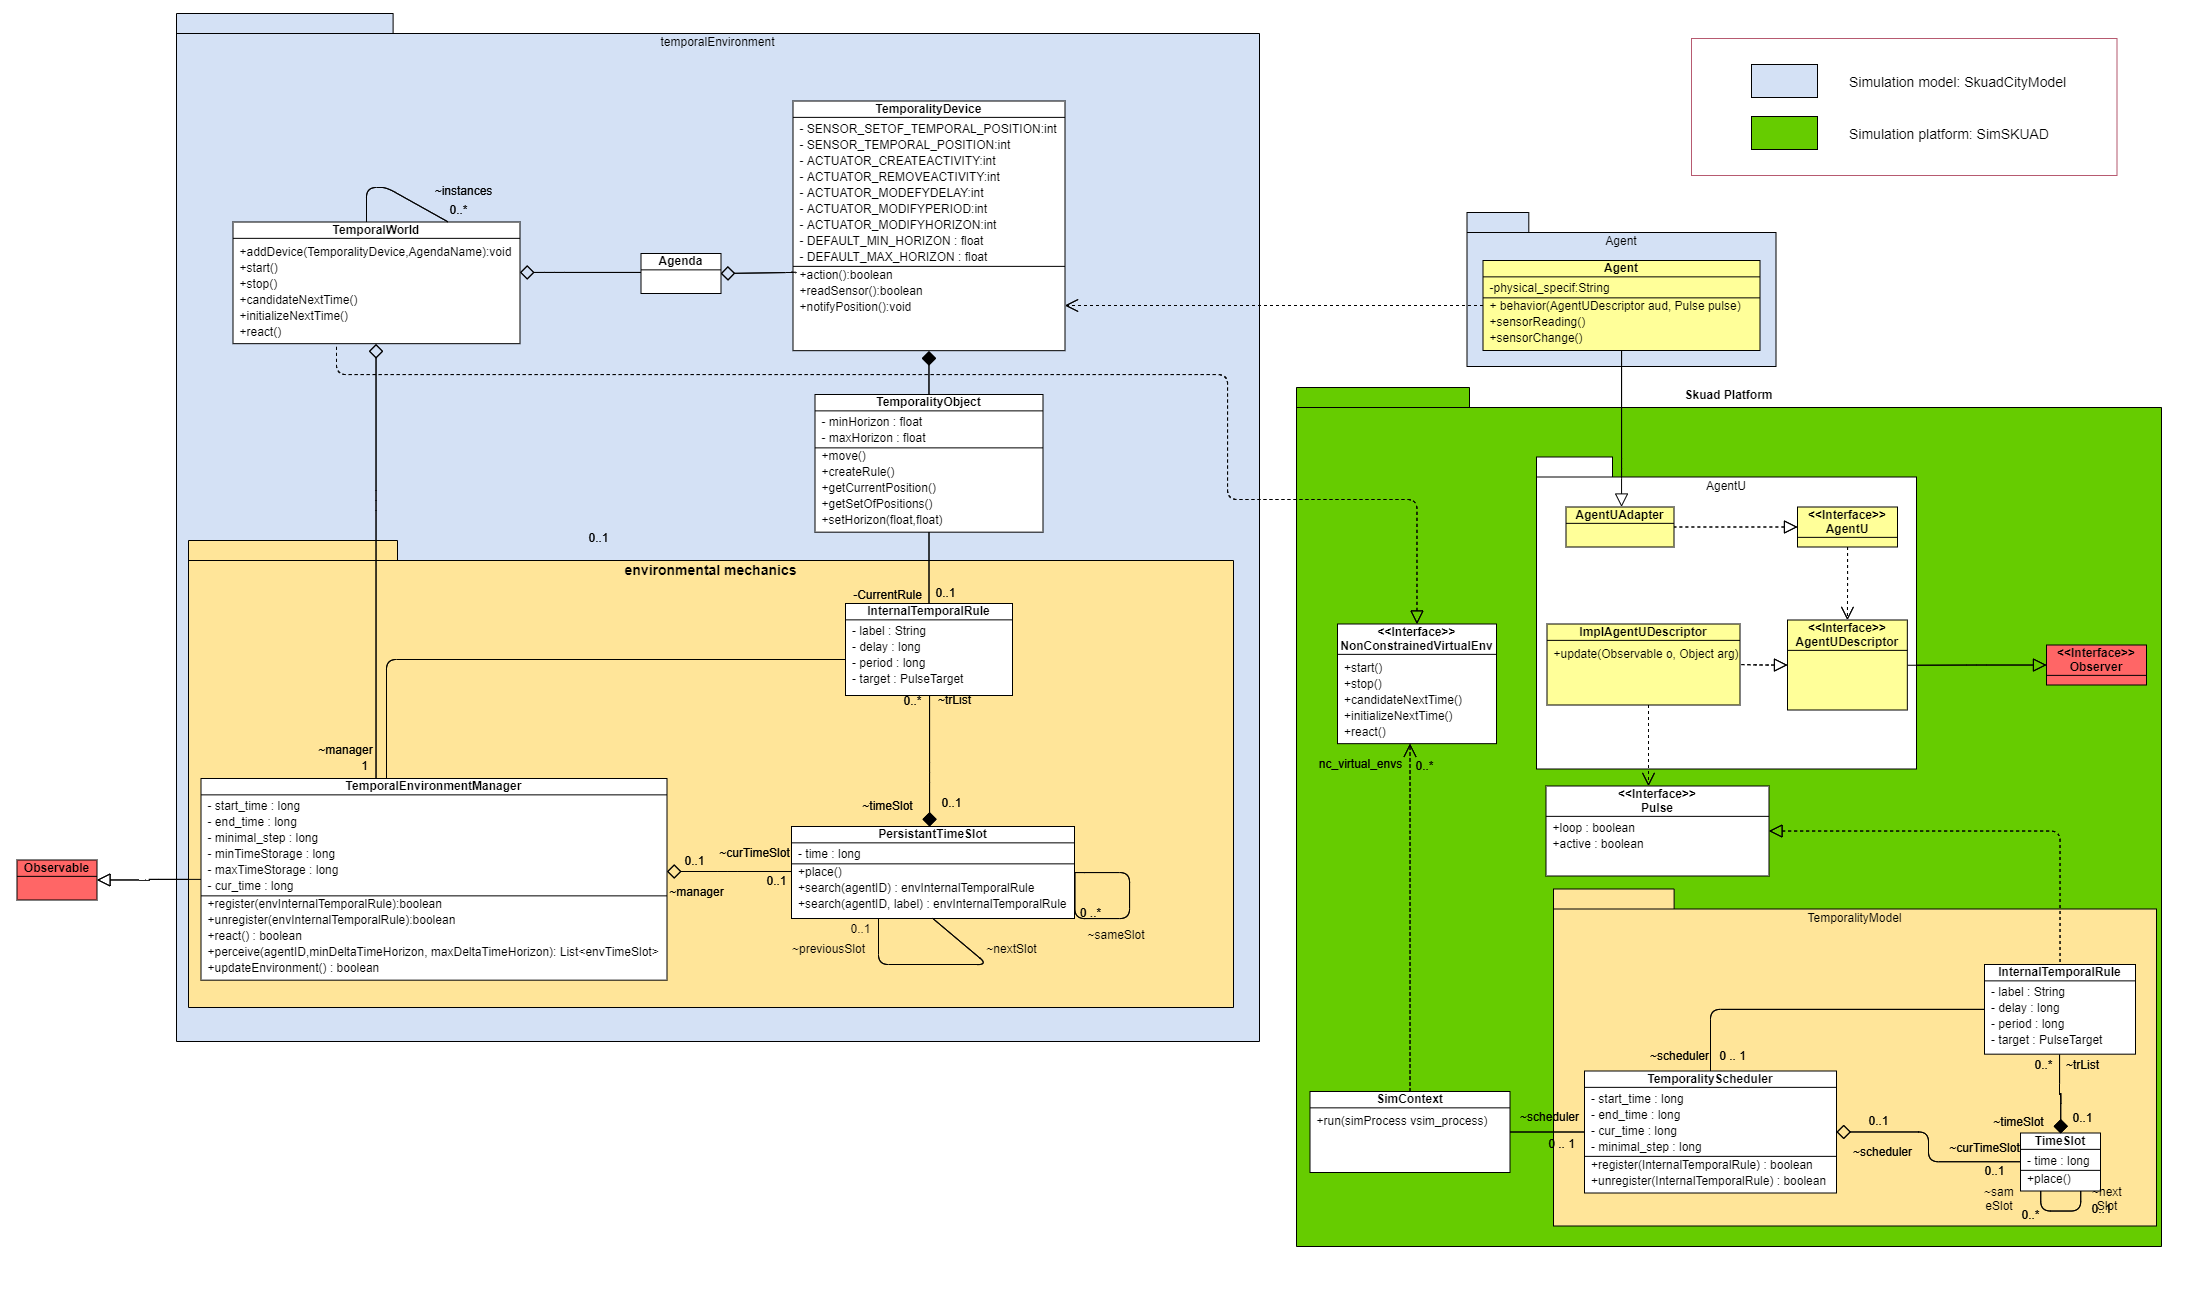
\includegraphics[width=\textwidth]{figures/temporalEnvironmentImpl.png}
	\end{figure}
\note{
Les mécaniques environnementaux qui reprennent les principes de base du modèle à temporalité. Comme vous pouvez le constater sur le schéma nous faisons le parallèle entre les mécaniques du modèle à temporalité utilisé au niveau de l’ordonnanceur et ceux ré-utilisés au niveau de l’environnement temporel. Nous pouvons notamment constater des différences par exemple au niveau de l’environnement temporel la possibilité de naviguer dans les 2 sens (vers le passé et vers le futur), la gestion du stockage, de la mise à jour, la réaction et la perception de l’environnement temporel.
\par Au niveau du modèle de simulation, notre implémentation de l’environnement temporel est assez générique pour être ré-utilisable facilement dans d’autres modèles de simulation tournant sur SimSKUAD.
\par De même les modifications effectuées au niveau de la plateforme de simulation ne devrait avoir aucune incidence sur les modèles de simulation déjà existantes tournant sur SimSKUAD.
}
    
\end{frame}